\documentclass{ucph-handout}
\usepackage{wrapfig}
\usepackage{fancyvrb}
\newcounter{handout}
\newcommand{\Ark}{Ark \#\arabic{handout} -- }
\renewcommand{\TimeAndLocation}{DIKU, 2021}%
\usepackage[bottom=3cm]{geometry}

\renewcommand{\Author}{Maja Hvidtfeldt Håkansson}
\renewcommand{\AuthorEmail}{mhv@di.ku.dk}

\begin{document}

\renewcommand{\Title}{\Ark LCD skærmen}

\begin{exercisebox}[adjusted title=De første skridt]
Åbn Mu-editoren og tilslut M5StickC via det medfølgende usb-kabel. Mu skulle gerne selv opdage M5StickC. Nederst i højre hjørne skal der stå: 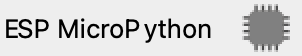
\includegraphics[width=0.20\textwidth]{ikoner/det.png}.\\ Når det er på plads er du klar til at gå videre.

\tcbsubtitle{Første program}

Slet den linje hvor der står \textit{\#Write your code here :-)} og skriv i stedet følgende linjer:

\begin{verbatim}
    1   from m5stack import lcd
    2
    3   lcd.orient(lcd.LANDSCAPE)
    4   lcd.clear(0xFF0000)
\end{verbatim}

tryk på \textbf{Run} 
\includegraphics[width=0.05\textwidth]{ikoner/run.png} og se hvad der sker. \\

Prøv at erstatte det der står i parantesen på linje 4 med 0x00FF00 og tryk på \textbf{Run} 
\includegraphics[width=0.05\textwidth]{ikoner/run.png}\\ 
Prøv det samme med 0x0000FF og 0xFFFF00\\

Kan du få skærmen til at blive lilla? Hvad med sort?

\textbf{TIP:} søg på "HEX color picker" på Google

\vspace{3mm}
\tcbsubtitle{Tekst på skærmen}
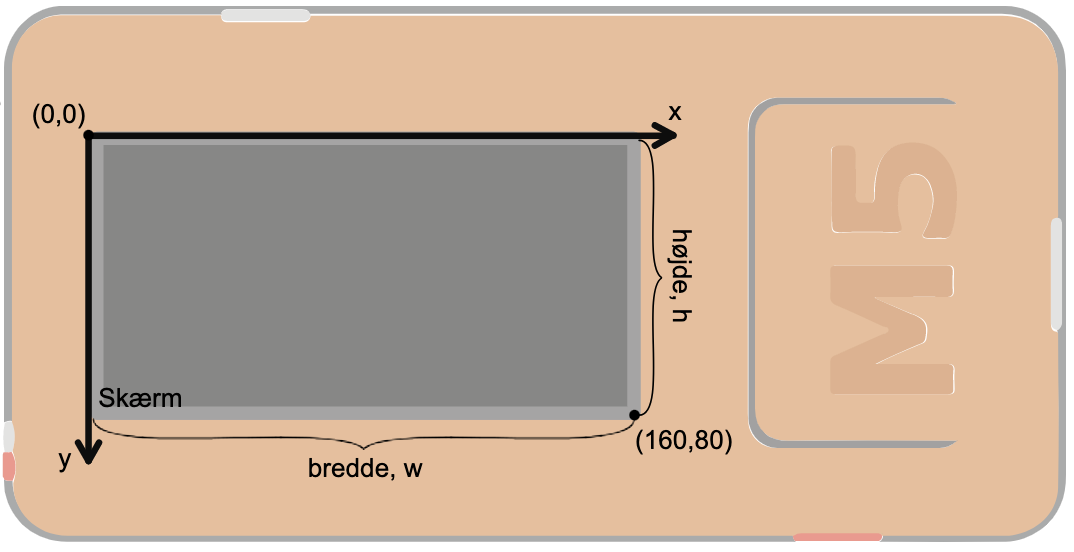
\includegraphics[width=0.6\textwidth]{billeder/landskabeorient.png}\\
For at placere tekst på skærmen skal vi give koordinaterne til hvor teksten skal placeres, sammen med den ønskede tekst. M5StickCs koordinatsystem vender lidt på hovedet i forhold til dem I kender fra matematik. Punktet (0,0) er i øverste venstre hjørne, og y-aksen vokser nedad. Men princippet er det samme; et punkt har et x og et y koordinat. \\

Tilføj en 5. linje til din kode hvor der står 
\begin{verbatim}
    5   lcd.text(10, 10, "Hello!")
\end{verbatim}

\vspace{3mm}

\tcbsubtitle{Øvelse}
\vspace{3mm}
Skriv dit navn på midten af skærmen! \\

Gem den kode du har lavet ved at trykke \textbf{Save} 
\includegraphics[width=0.05\textwidth]{ikoner/save.png}. Giv din kode navnet "lcd.py"
\vspace{3mm}

\end{exercisebox}

\newpage
\begin{exercisebox}[adjusted title= Tegning]
Man kan også tegne figurer og linjer på skærmen. \\
Klik på \textbf{New} 
\includegraphics[width=0.05\textwidth]{ikoner/new.png} for at begynde en ny kode. \\

Slet den linje hvor der står \textit{\#Write your code here :-)} og skriv i stedet følgende linjer:\\
\begin{verbatim}
    1   from m5stack import lcd
    2
    3   lcd.orient(lcd.LANDSCAPE)
    4   lcd.clear(0xFFFFFF)
    5
    6   lcd.circle(40, 50, 30, fillcolor=0xffcf00)
    7   lcd.line(25,60,55,60,color=0x000000)
    8
    9   lcd.circle(30, 40, 10, fillcolor=0xFFFFFF)
    10  lcd.circle(50, 40, 10, fillcolor=0xFFFFFF)
    11  lcd.circle(30, 43, 4, fillcolor=0x000000)
    12  lcd.circle(50, 43, 4, fillcolor=0x000000)
\end{verbatim}

Tryk på \textbf{Run} 
\includegraphics[width=0.05\textwidth]{ikoner/run.png}\\

Man kan farve sine figurer på med \textbf{color} og \textbf{fillcolor}. \textbf{Color} er farven man vil have stregen, eller omridset skal have. \textbf{Fillcolor} er hvad figuren skal fyldes med.\\

Hvis man f.eks. skrev: \textit{lcd.circle(40, 40, 30, color=0xFF0000, fillcolor=0xFFCF00)} ville man få en gul cirkel med et rødt omrids.\\

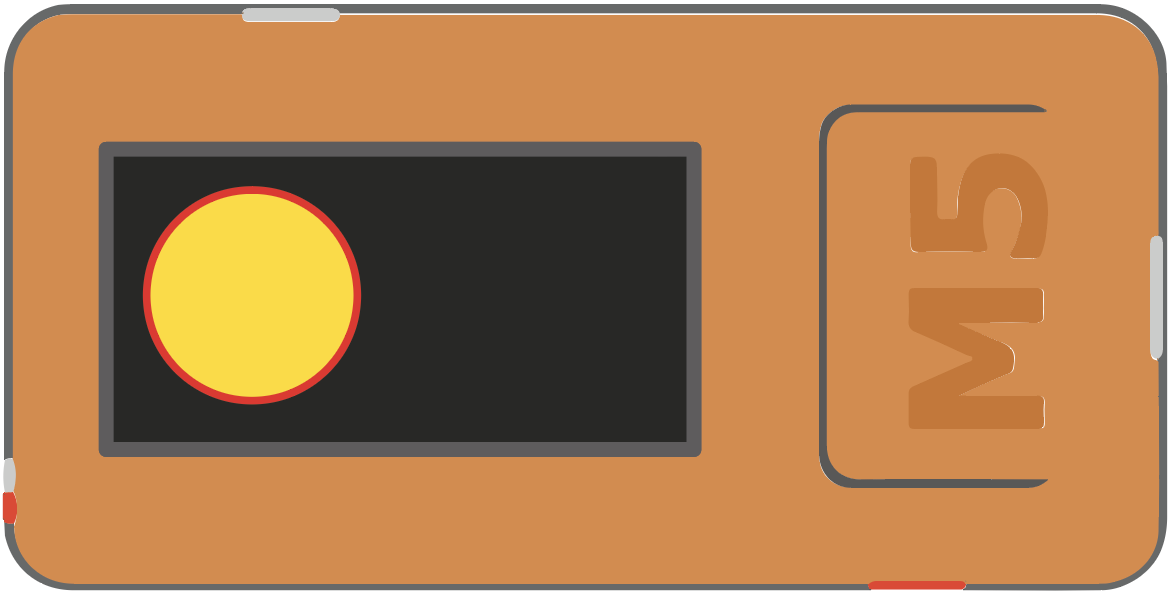
\includegraphics[width=0.5\textwidth]{billeder/cirkel.png}\\

Hvis man ikke skriver nogen fillcolor, får man bare et omrids.\\

\tcbsubtitle{Øvelse}
\vspace{3mm}
Tegn endnu et ansigt i højre side af skærmen. \\

Gem den kode du har lavet ved at trykke \textbf{Save} 
\includegraphics[width=0.05\textwidth]{ikoner/save.png}. Giv din kode navnet "emoji.py"\\\\
\textbf{Tip:} På \url{https://m5guide.readthedocs.io/da/latest/tegne.html} kan I finde hjælp til at tegne figurer og farve dem.

\end{exercisebox}


\newpage
\stepcounter{handout}
\renewcommand{\Title}{\Ark IMU/bevægelsessensor}
\begin{exercisebox}[adjusted title=Bevægelsessensor]
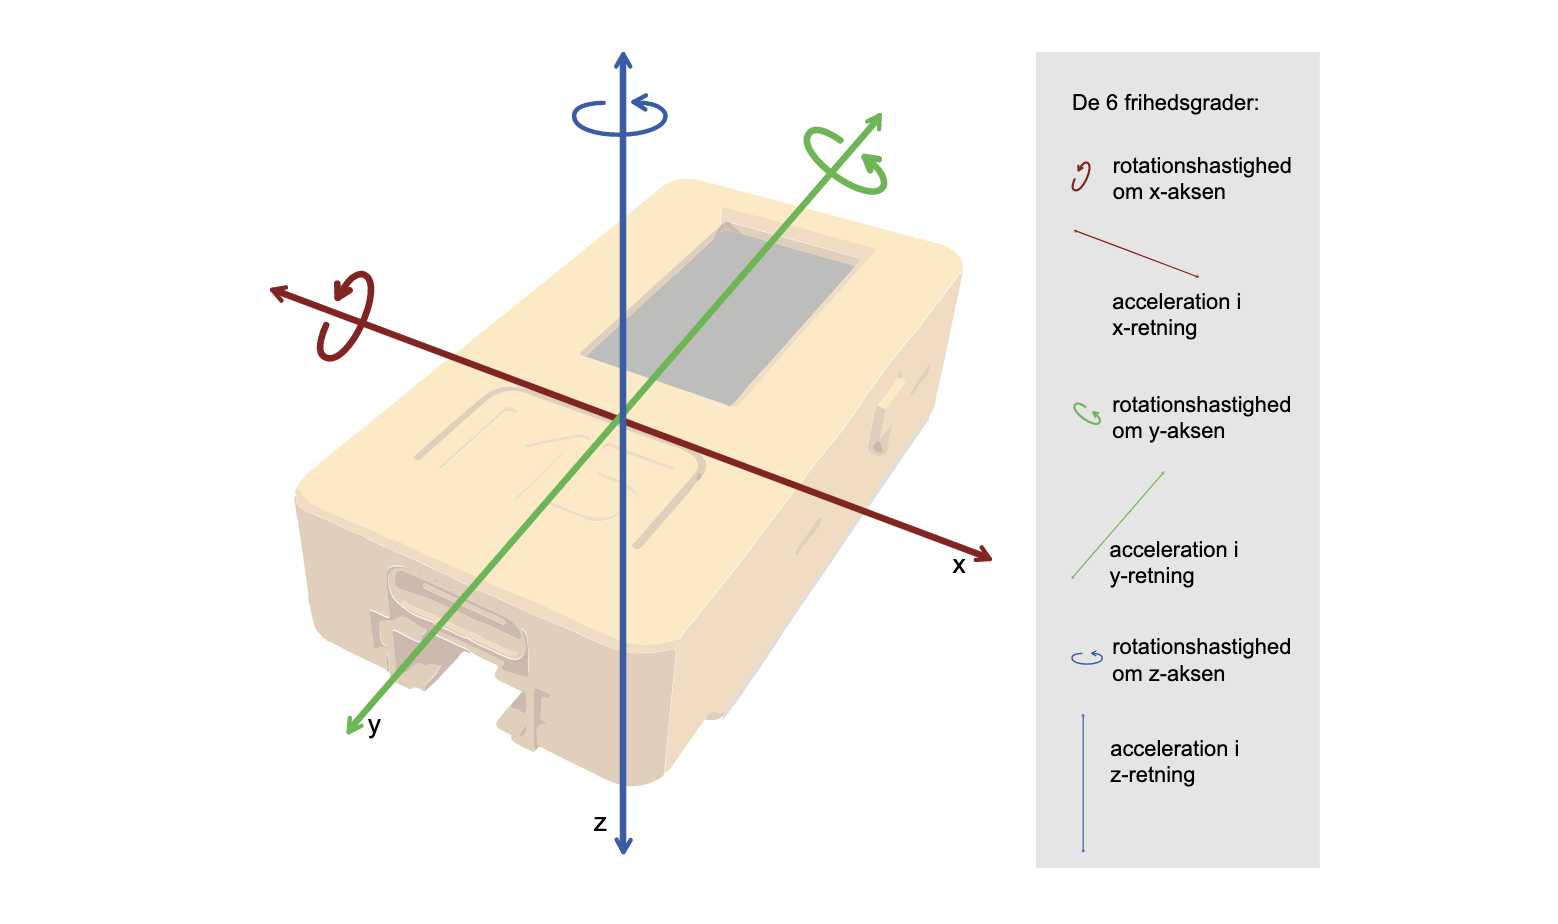
\includegraphics[width=0.9\textwidth]{billeder/aaccel.png}\\
M5StickC har en indbygget bevægelsessensor, kaldet en \textbf{IMU}, og den skal vi bruge. \\
Klik på \textbf{New} 
\includegraphics[width=0.05\textwidth]{ikoner/new.png} for at begynde en ny kode. \\

Slet den linje hvor der står \textit{\#Write your code here :-)} og skriv i stedet følgende:
\begin{verbatim}
    1   import imu
    2   sensor = imu.IMU()
    3
    4   while True:
    5       print(sensor.acceleration)
\end{verbatim}

Klik på \textbf{Run} 
\includegraphics[width=0.05\textwidth]{ikoner/run.png} og derefter på \textbf{Plotter}  
\includegraphics[width=0.05\textwidth]{ikoner/poltter.png}.\\

\tcbsubtitle{Øvelse - acceleration}
Prøv at lade den ligge stille, fladt på bordet. Prøv at vende den så den står på højkant og på siden. Bevæg den lidt. Kan du regne ud hvad den måler? Skriv dit bedste bud herunder. \\
\textit{(Undgå at skrive det åbenlyse: "acceleration" - overvej hvad acceleration egentlig betyder)}\\\\

sensor.acceleration måler: \rule{8cm}{0.4pt}

\tcbsubtitle{Øvelse - gyroskop}
Erstat linje 5 med:
\begin{verbatim}
    5       print(sensor.gyro)
\end{verbatim}
\\~\\
Klik på \textbf{Run} 
\includegraphics[width=0.05\textwidth]{ikoner/run.png} og derefter på \textbf{Plotter}. Prøv at bevæge M5StickC og se om du kan regne ud hvad den måler? Skriv dit bedste bud herunder.\\

sensor.gyro måler: \rule{8cm}{0.4pt}

\end{exercisebox}
\newpage
\begin{exercisebox}[adjusted title=Pitch og Roll]

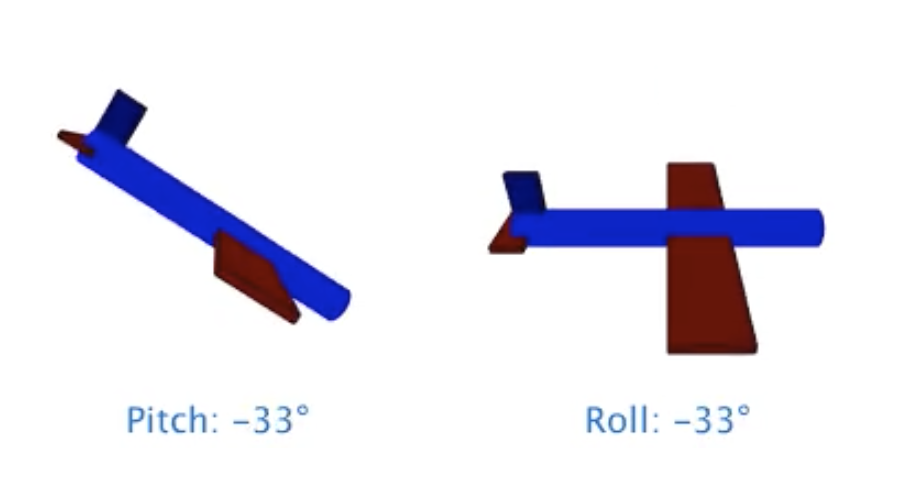
\includegraphics[width=0.5\textwidth]{billeder/pitchroll.png}

De rå data fra IMU'en er lidt svære at aflæse, men hvis man kombinere accelometerdata med gyroskopdata, kan man regne det der hedder \textit{pitch} og \textit{roll} ud. \\
Hvis man tænker på et fly, så er pitch et udtryk for hvad vej spidsen af flyet peger, mens roll er et udtryk for hvor meget flyet har roteret. \\

Klik på \textbf{New} 
\includegraphics[width=0.05\textwidth]{ikoner/new.png} for at begynde en ny kode og skriv:

\begin{verbatim}
    1   from m5stack import lcd
    2   import imu
    3   import fusion
    4
    5   myIMU = imu.IMU()   
    6   filter = fusion.MahonyFilter()
    7   lcd.orient(lcd.LANDSCAPE)
    8
    9   while True:
   10        filter.update(myIMU.acceleration, myIMU.gyro)
   11        pitch = str(int(filter.pitch))
   12        roll = str(int(filter.roll))
   13        print("pitch: " + pitch + " roll: " + roll)
\end{verbatim}
Klik på \textbf{Run} 
\includegraphics[width=0.05\textwidth]{ikoner/run.png}\\

Lige nu bliver pitch og roll skrevet ud i Mu - men vi vil gerne kunne aflæse det på M5StickC.
\tcbsubtitle{Opgave}

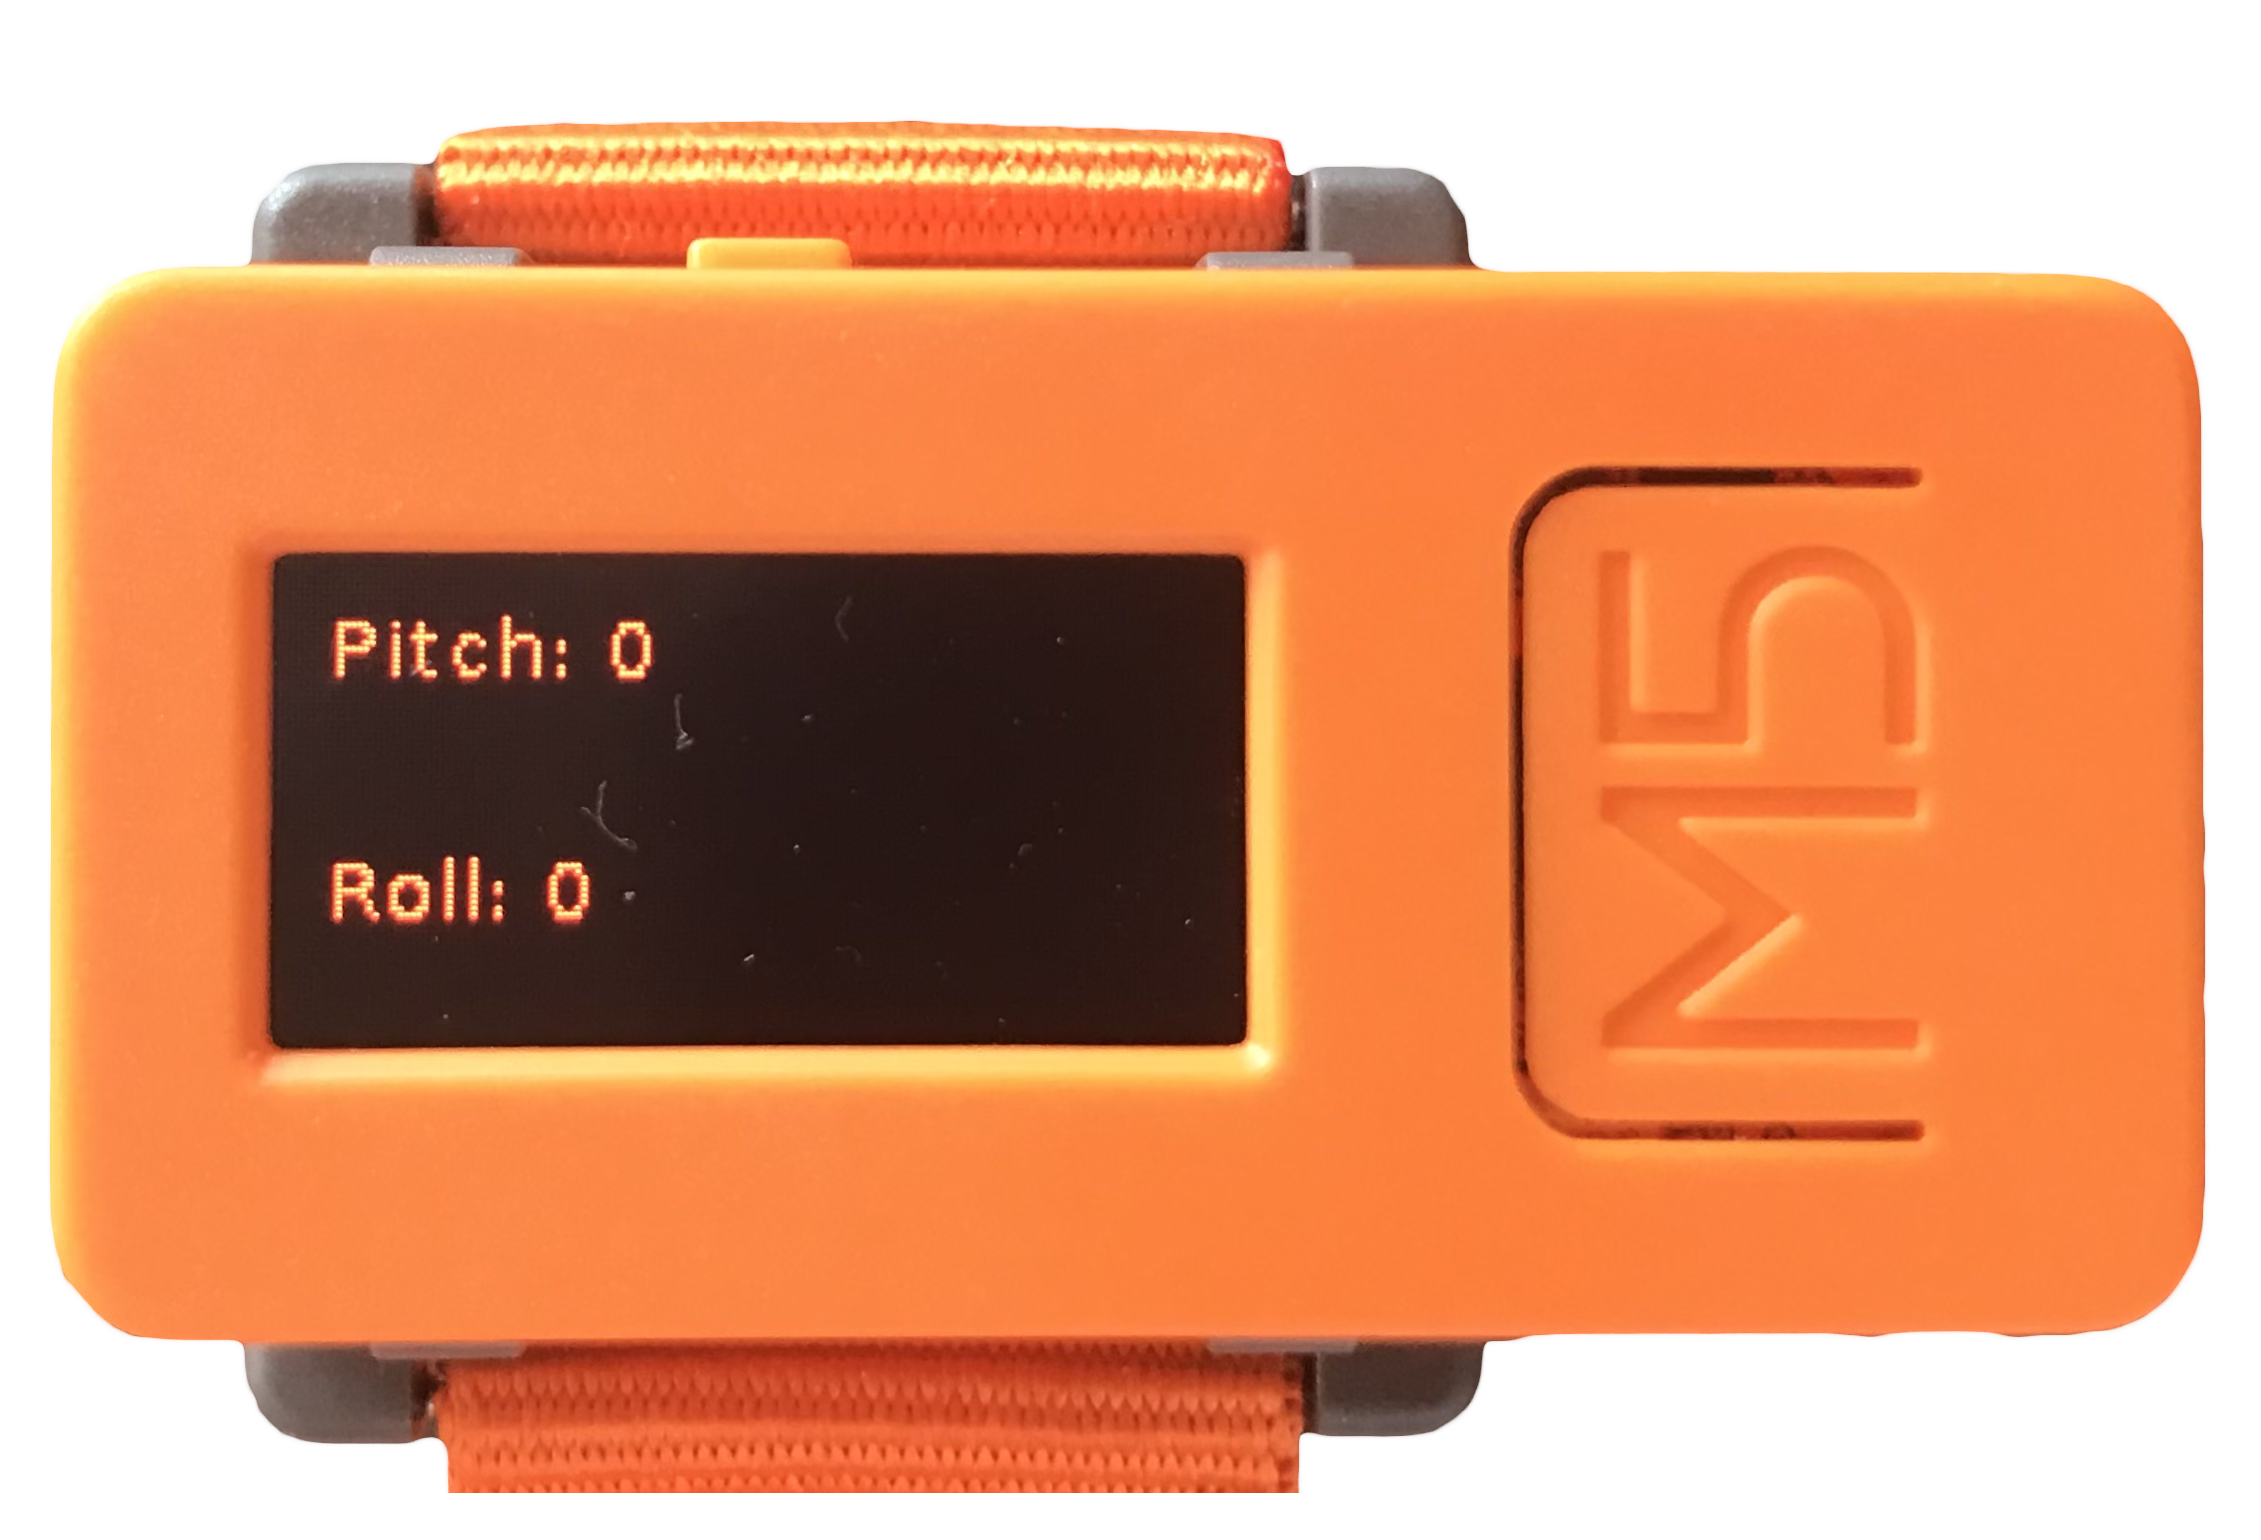
\includegraphics[width=0.4\textwidth]{billeder/pitchrollbillede.png}

Forsøg ved hjælp af \url{lcd.text}, om du kan skrive noget kode, så man kan aflæse pitch og roll på uret. \\

Du kan starte på linje 14, sådan her:
\begin{verbatim}
   14       lcd.text(10, 10, "Pitch:")
\end{verbatim}

\end{exercisebox}

\newpage

\stepcounter{handout}
\renewcommand{\Title}{\Ark Lyd og lyt}
\begin{exercisebox}[adjusted title=Højtaler]

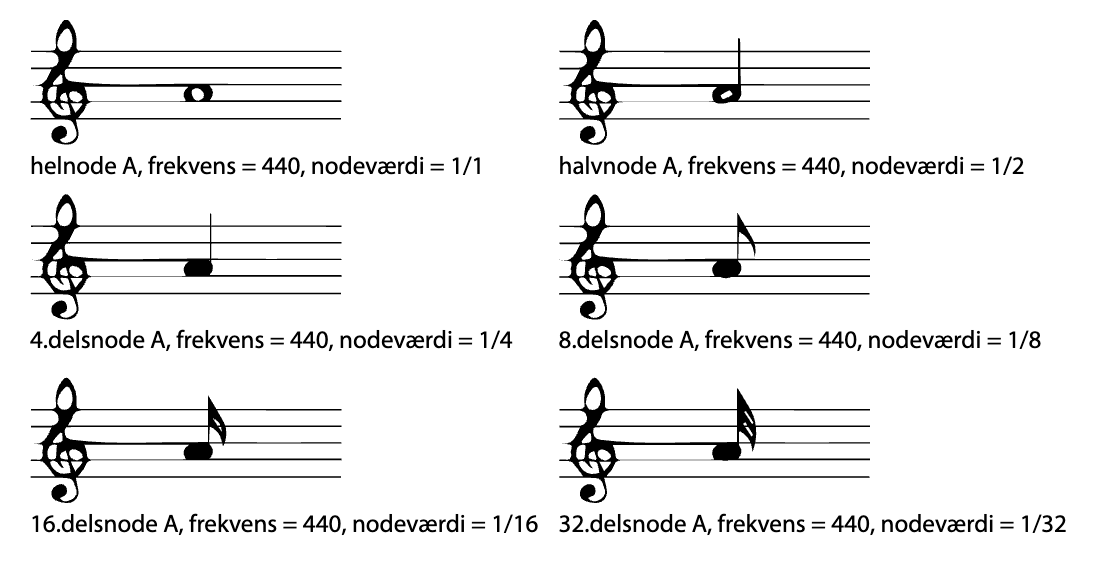
\includegraphics[width=0.6\textwidth]{billeder/toner.png}

Klik på \textbf{New}

\includegraphics[width=0.05\textwidth]{ikoner/new.png} for at begynde en ny kode og skriv:

\begin{verbatim}
    1   from m5stack import lcd
    2   from flowlib import hat
    3   import time
    4
    5   spk = hat.get(hat.SPEAKER)
    6
    7   spk.sing(440, 1/4)
    8   time.sleep_ms(100)
    9   spk.sing(440, 1/4)
\end{verbatim}

Klik på \textbf{Run} 
\includegraphics[width=0.05\textwidth]{ikoner/run.png}. \\

Den tone du hører er kammertonen "A". Tonens frekvens er 440 Hz, og nodeværdien er $\frac{1}{4}$ og det er netop de to ting vi har brug for at bestemme, for at få afspillet en tone. \\

\tcbsubtitle{Opgave}

Starten af Lille Peter Edderkop kan spilles ved hjælp af 3 toner; et \textbf{C} et \textbf{D} og et \textbf{E}.\\

Den starter på \textbf{C}.\\

Tonen C har en frekvens på \textbf{523} Hz, D har en frekvens på \textbf{587} Hz og E har en frekvens på \textbf{659} Hz. \\

Hvor langt kan du komme i sangen?\\

\begin{verbatim}
    C  C  C D   E E  E
    Lille Peter Edderkop
    D   D    D  E  C C 
    Kravled' op ad muren
\end{verbatim}\\

\textbf{Lyst til mere musik?} Du kan finde en oversigt over alle tonernes frekvenser her:\\
\nolinkurl{https://m5guide.readthedocs.io/da/latest/hat.html#frek}

\end{exercisebox}
\newpage
\begin{exercisebox}[adjusted title=Kode til overvågning]

Gå ind på \url{https://github.com/Majahh/smartwatch/blob/main/coronaalarm.py}\\
Marker \textbf{al} koden og kopier ved at trykke ctrl+c. Åben en ny fil i Mu \textbf{New} 
\includegraphics[width=0.05\textwidth]{ikoner/new.png} og indsæt alt det du har kopieret ved at trykke ctrl+v\\

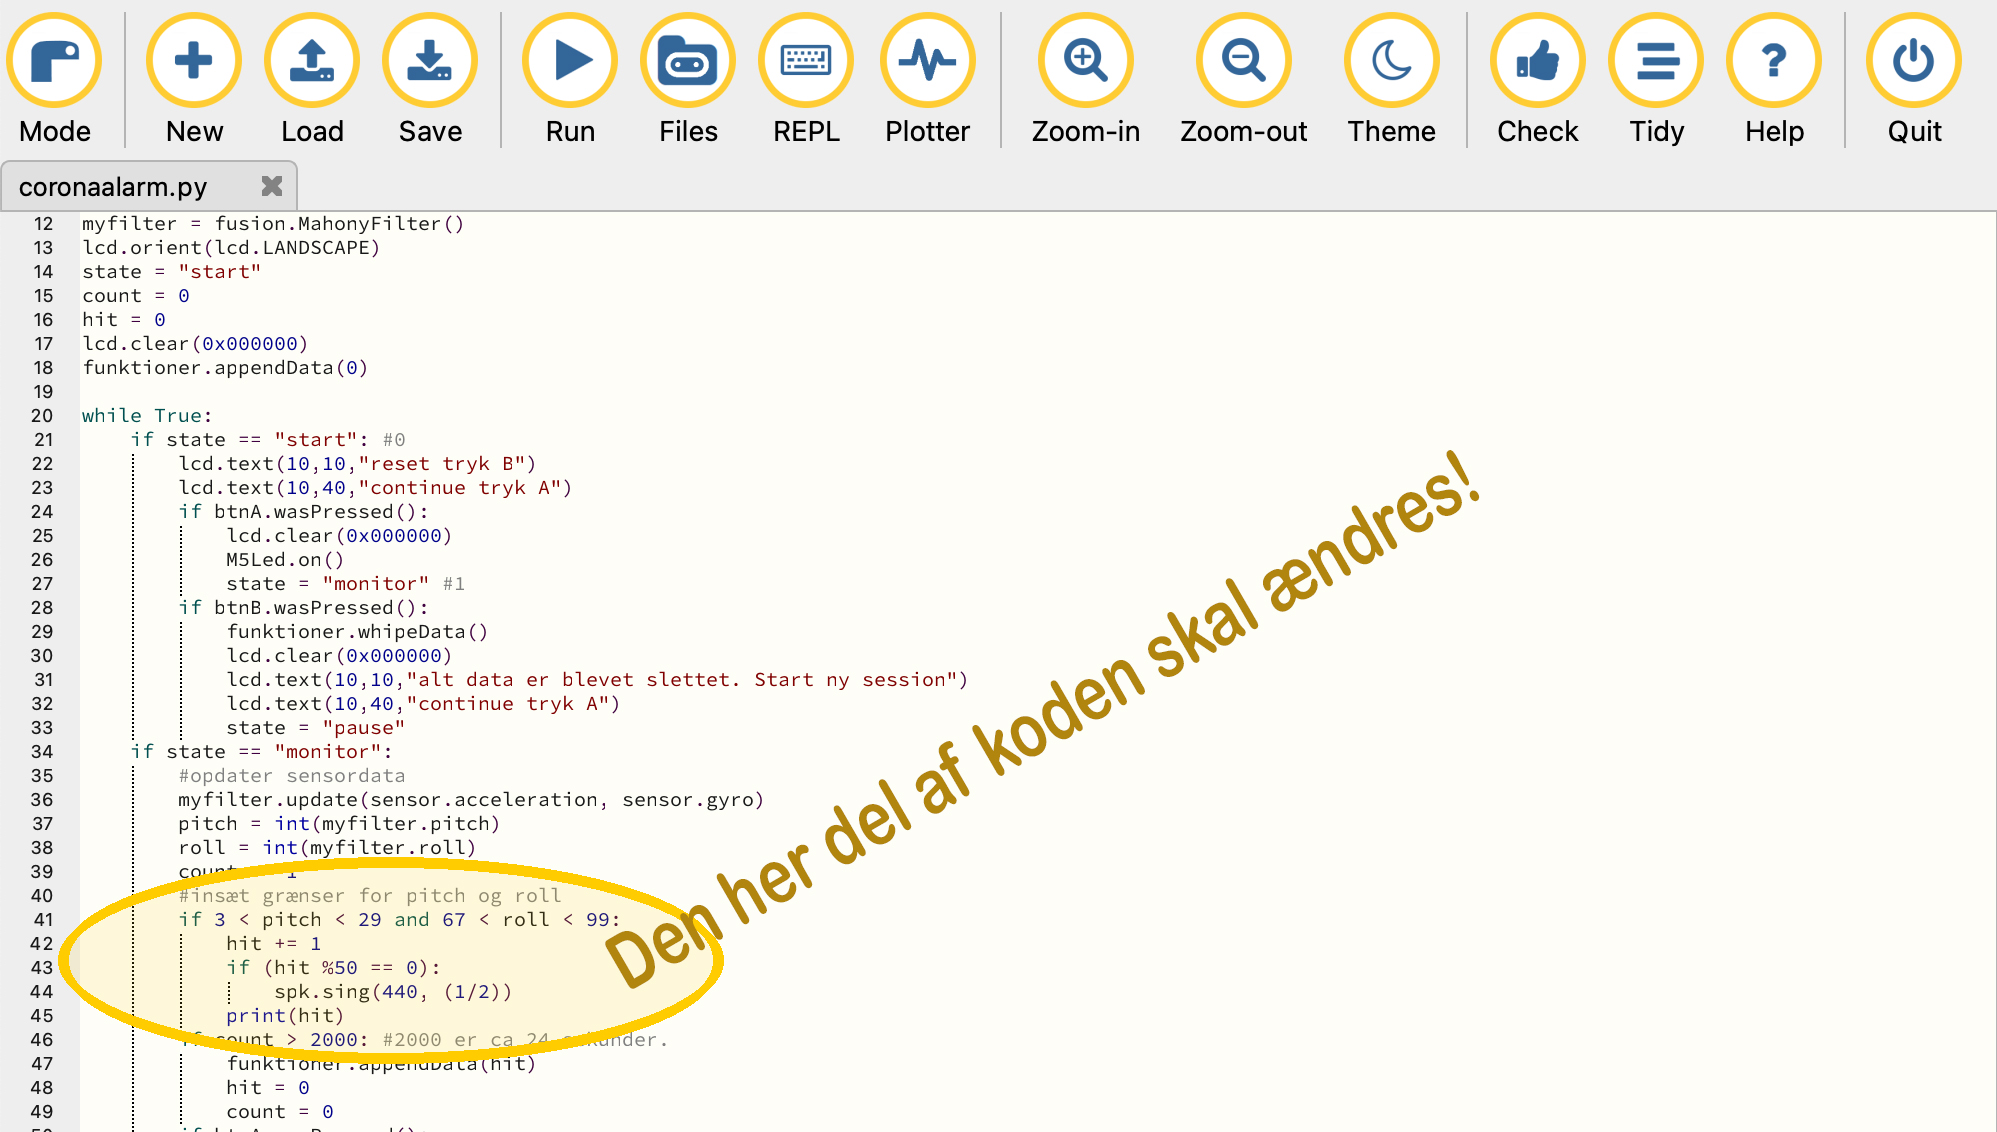
\includegraphics[width=1\textwidth]{billeder/and.jpg}\\

Jeres egne fundne grænser for pitch og roll sættes ind på den linje  hvor der står :
\begin{verbatim}
    if 3 < pitch < 29 and 67 < roll < 99:
\end{verbatim}

\tcbsubtitle{Øvelse}
Læs koden igennem og finde de steder I kan personliggøre koden - I kan ændre i den tekst der bliver skrevet på skærmen eller på farverne. Kig efter \url{lcd.text} og Hexidecimaltal ala 0x0F00FFF\\ Husk at trykke \textbf{Run} 
\includegraphics[width=0.05\textwidth]{ikoner/run.png}, hver gang i har ændret i koden for at tjekke at det stadig kan køres (og for at se om jeres ændring virkede).

\tcbsubtitle{Overfør koden til uret}

For at kunne køre koden selvstændig på uret, uden det er tilsluttet computer, skal det overføres til uret.\\
Først skal du gemme din kode - tryk \textbf{Save} 
\includegraphics[width=0.05\textwidth]{ikoner/save.png}. Giv din kode navnet "mobilemonitor.py". Sørg for at REPL er lukket ved at klikke på \textbf{REPL} 
\includegraphics[width=0.05\textwidth]{ikoner/REPL.png}. Nu kan du åbne for filerne, der ligger på din M5StickC. Klik på \textbf{Files} 
\includegraphics[width=0.05\textwidth]{ikoner/files.png}\\

Til højre ser du en liste med filer gemt på computeren - højreklik på filen "mobilemonitor.py" og vælg "Write to main.py on device". \\

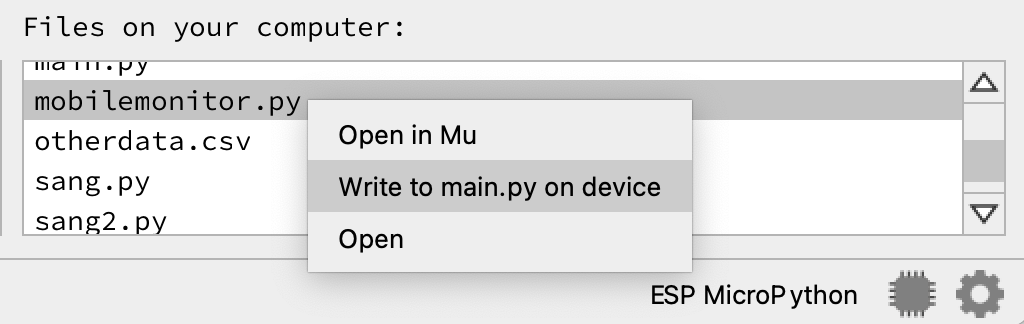
\includegraphics[width=0.50\textwidth]{billeder/wwritetomain.png}

\end{exercisebox}

\newpage

\stepcounter{handout}
\renewcommand{\Title}{\Ark Opgaven hjemme}
\begin{exercisebox}[adjusted title=Forberedelse]
Her er de 5 skridt I skal tage for at sætte det hele igang:
\begin{itemize}
    \item Oplad uret
    \item Lad forsøgpersonen læse bagsiden af dette ark.
    \item Påsæt uret på den hånd I har lavet programmet til og sørg for at det sidder stramt
    \item Start uret - den røde led lampe skal lyse.
    \item Sæt alarm/tidtagning til en time på din mobil
\end{itemize}

\tcbsubtitle{Udførsel}

Når uret sidder på personen, skal du prøve at undgå at blande dig, så personen ikke føler sig direkte overvåget\\

Hvis uret løber tør for strøm undervejs (den røde led slukker), så stop tidtagningen og lad uret op. Næste gang uret startes vælges "continue" og eksperimentet kan færdiggøres. Noter tiderne på arket\\

Når tiden er gået: tag gerne et billede af M5StickCs display med din mobil, så I har en backup, hvis uret løbet tør for strøm, eller I kommer til at slette data.\\ 
\tcbsubtitle{Aflæsning af opsamlede data}

Brug nu det udleverede ark til at få gang i en diskussion om data. Udfyld de ting der skal udfyldes og overvej, for hvert spørgsmål, hvad der taler for/imod det der svares. 

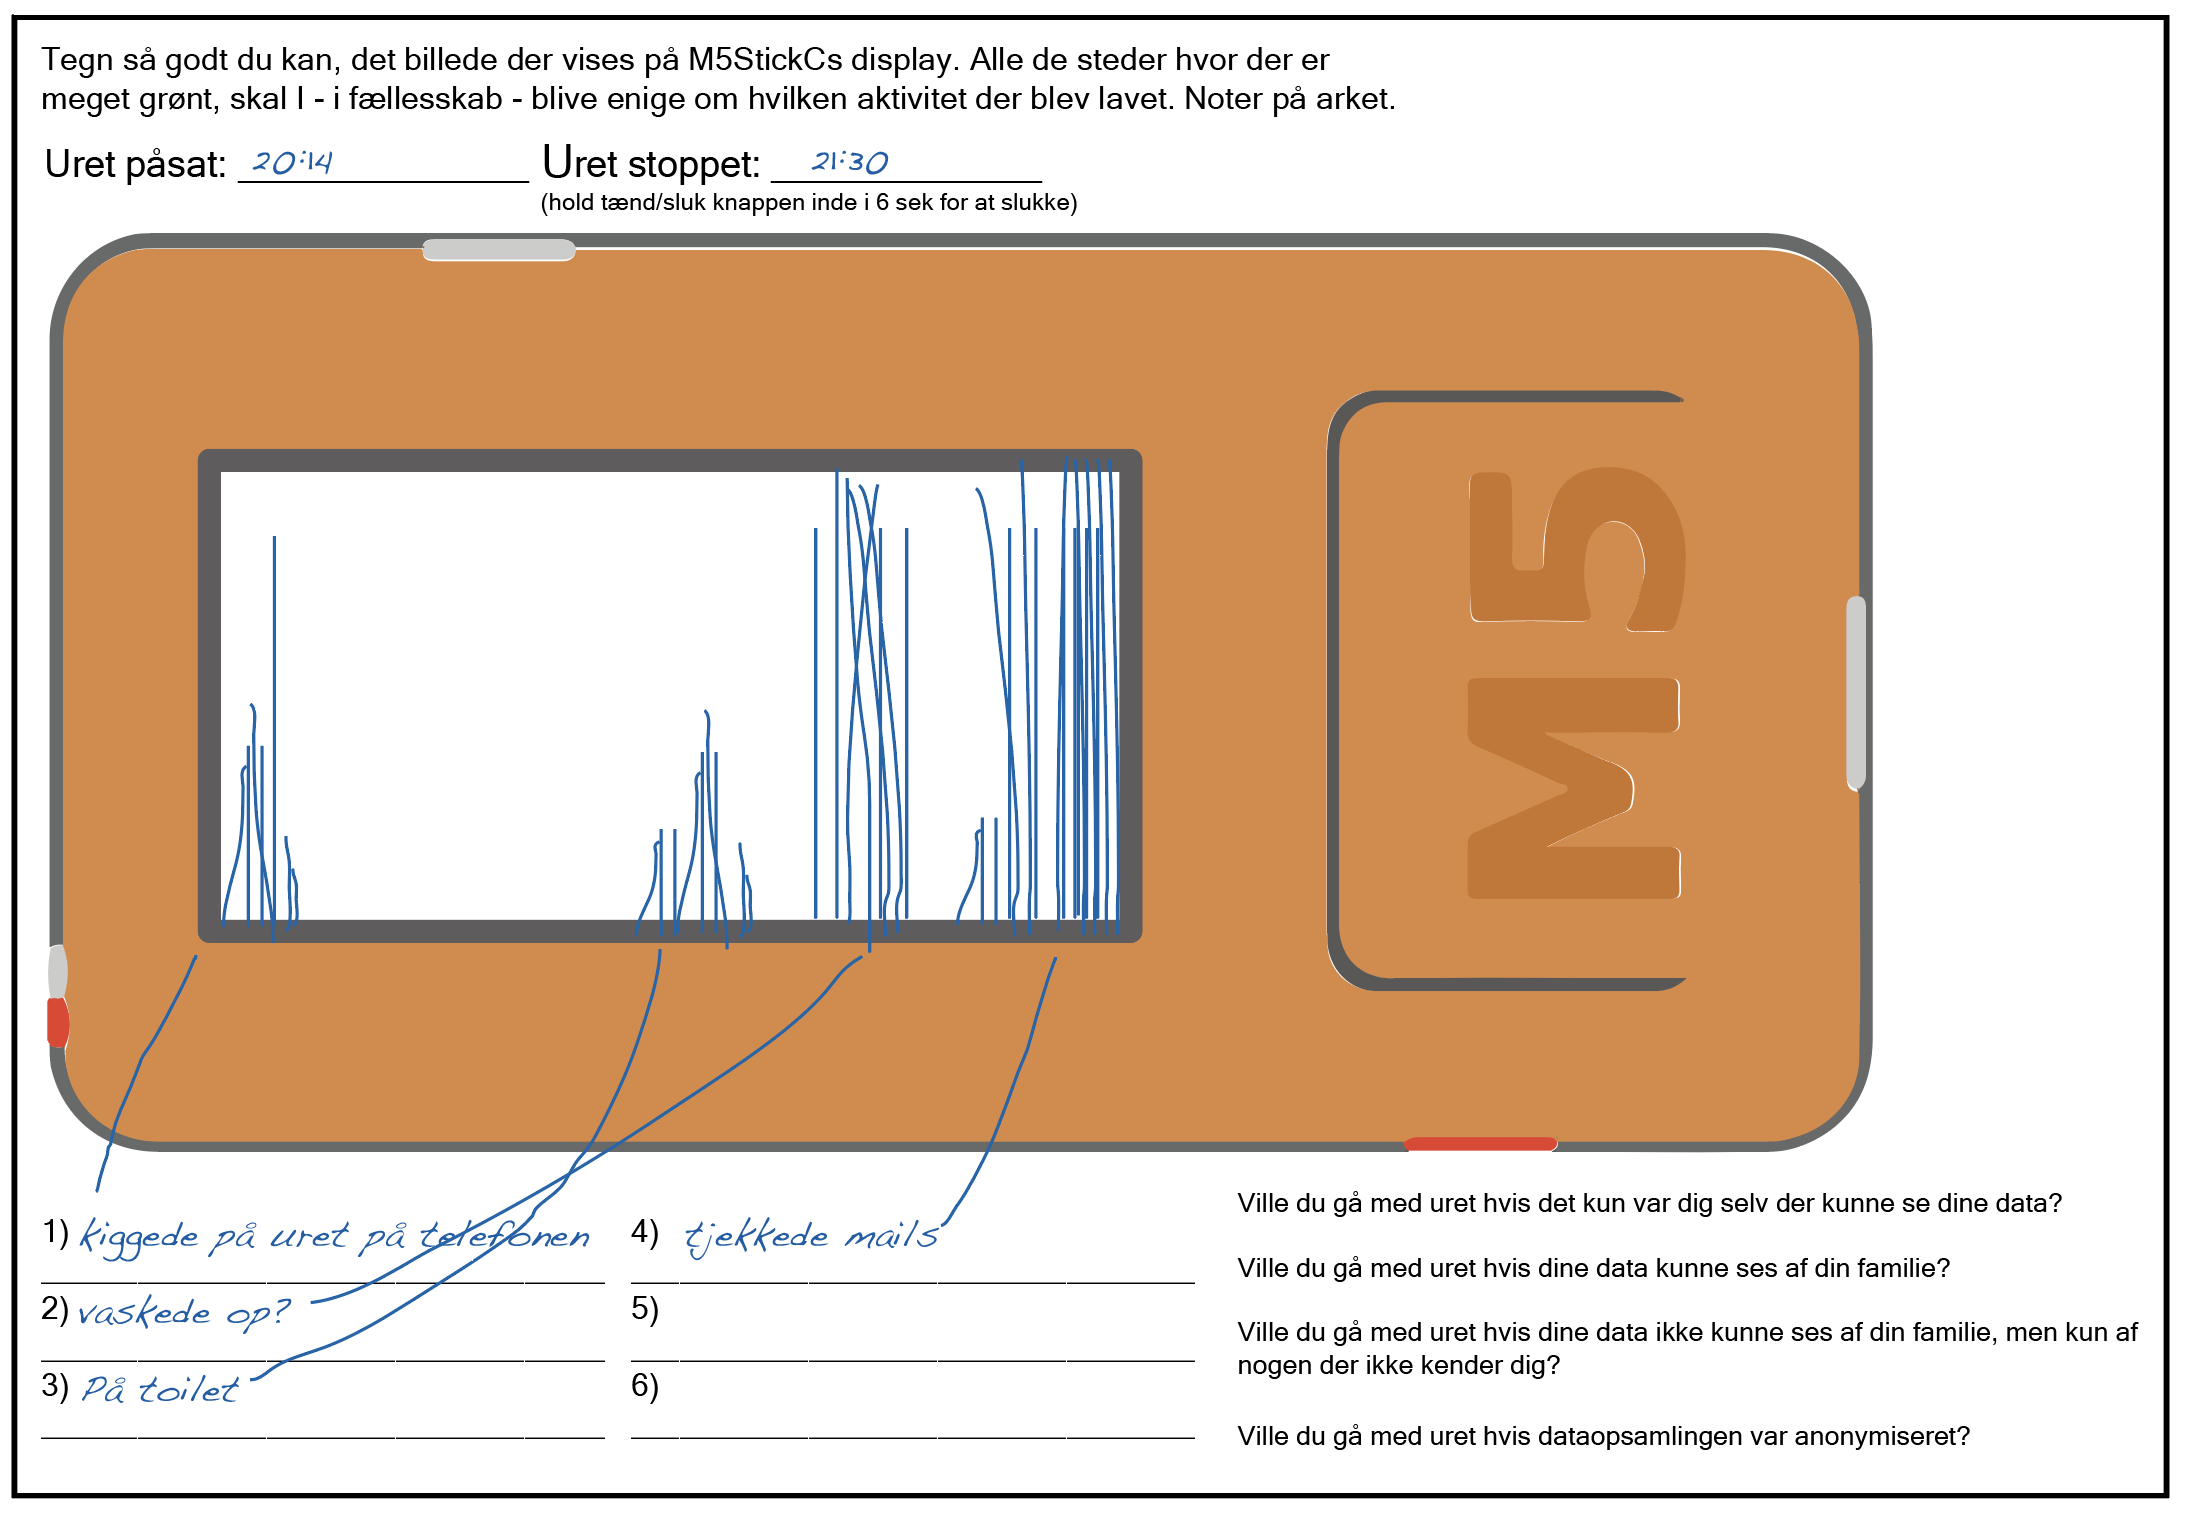
\includegraphics[width=0.9\textwidth]{billeder/udfyldtsp.png}

Hvis noget driller eller ikke vil virke, så ta' det helt roligt og prøv eventuelt at gentage eksperimentet. Hvis din forsøgsperson ikke synes det er sjovt at være med, så skal du også bare stoppe. \\

\textbf{Når I er færdige med opgaven lægger I det udfyldte ark i tasken - så har I det automatisk med næste gang vi ses!}
\end{exercisebox}

\begin{exercisebox}[adjusted title=Til forsøgspersonen:]

\textit{Dette er et forsøgsprojekt på Datalogisk Institut på Københavns Universitet der sætte fokus på data, overvågning og etik - med det mere specifikke formål at finde en relevant og vedkommende måde at undervise folkeskoleelever i emnet.} \\

\textit{De data der bliver indsamlet her bliver ikke gemt nogen steder.}\\

\textit{Det er meningen eksperimentet skal sætte gang i en debat mellem forældre og unge om dataovervågning og etik. Hvis det undervejs føles ubehageligt at blive overvåget, skal I bare stoppe eksperimentet og i stedet snakke om hvorfor I stoppede det.}\\ 

\textit{I er velkomne til at kontakte Maja Hvidtfeldt Håkansson på mhv@di.ku.dk ved spørgsmål}\\ 


\end{exercisebox}

\newpage

\stepcounter{handout}
\renewcommand{\Title}{\Ark frasorterede ark}

\begin{exercisebox}[adjusted title=Aflæs koordinaterne]

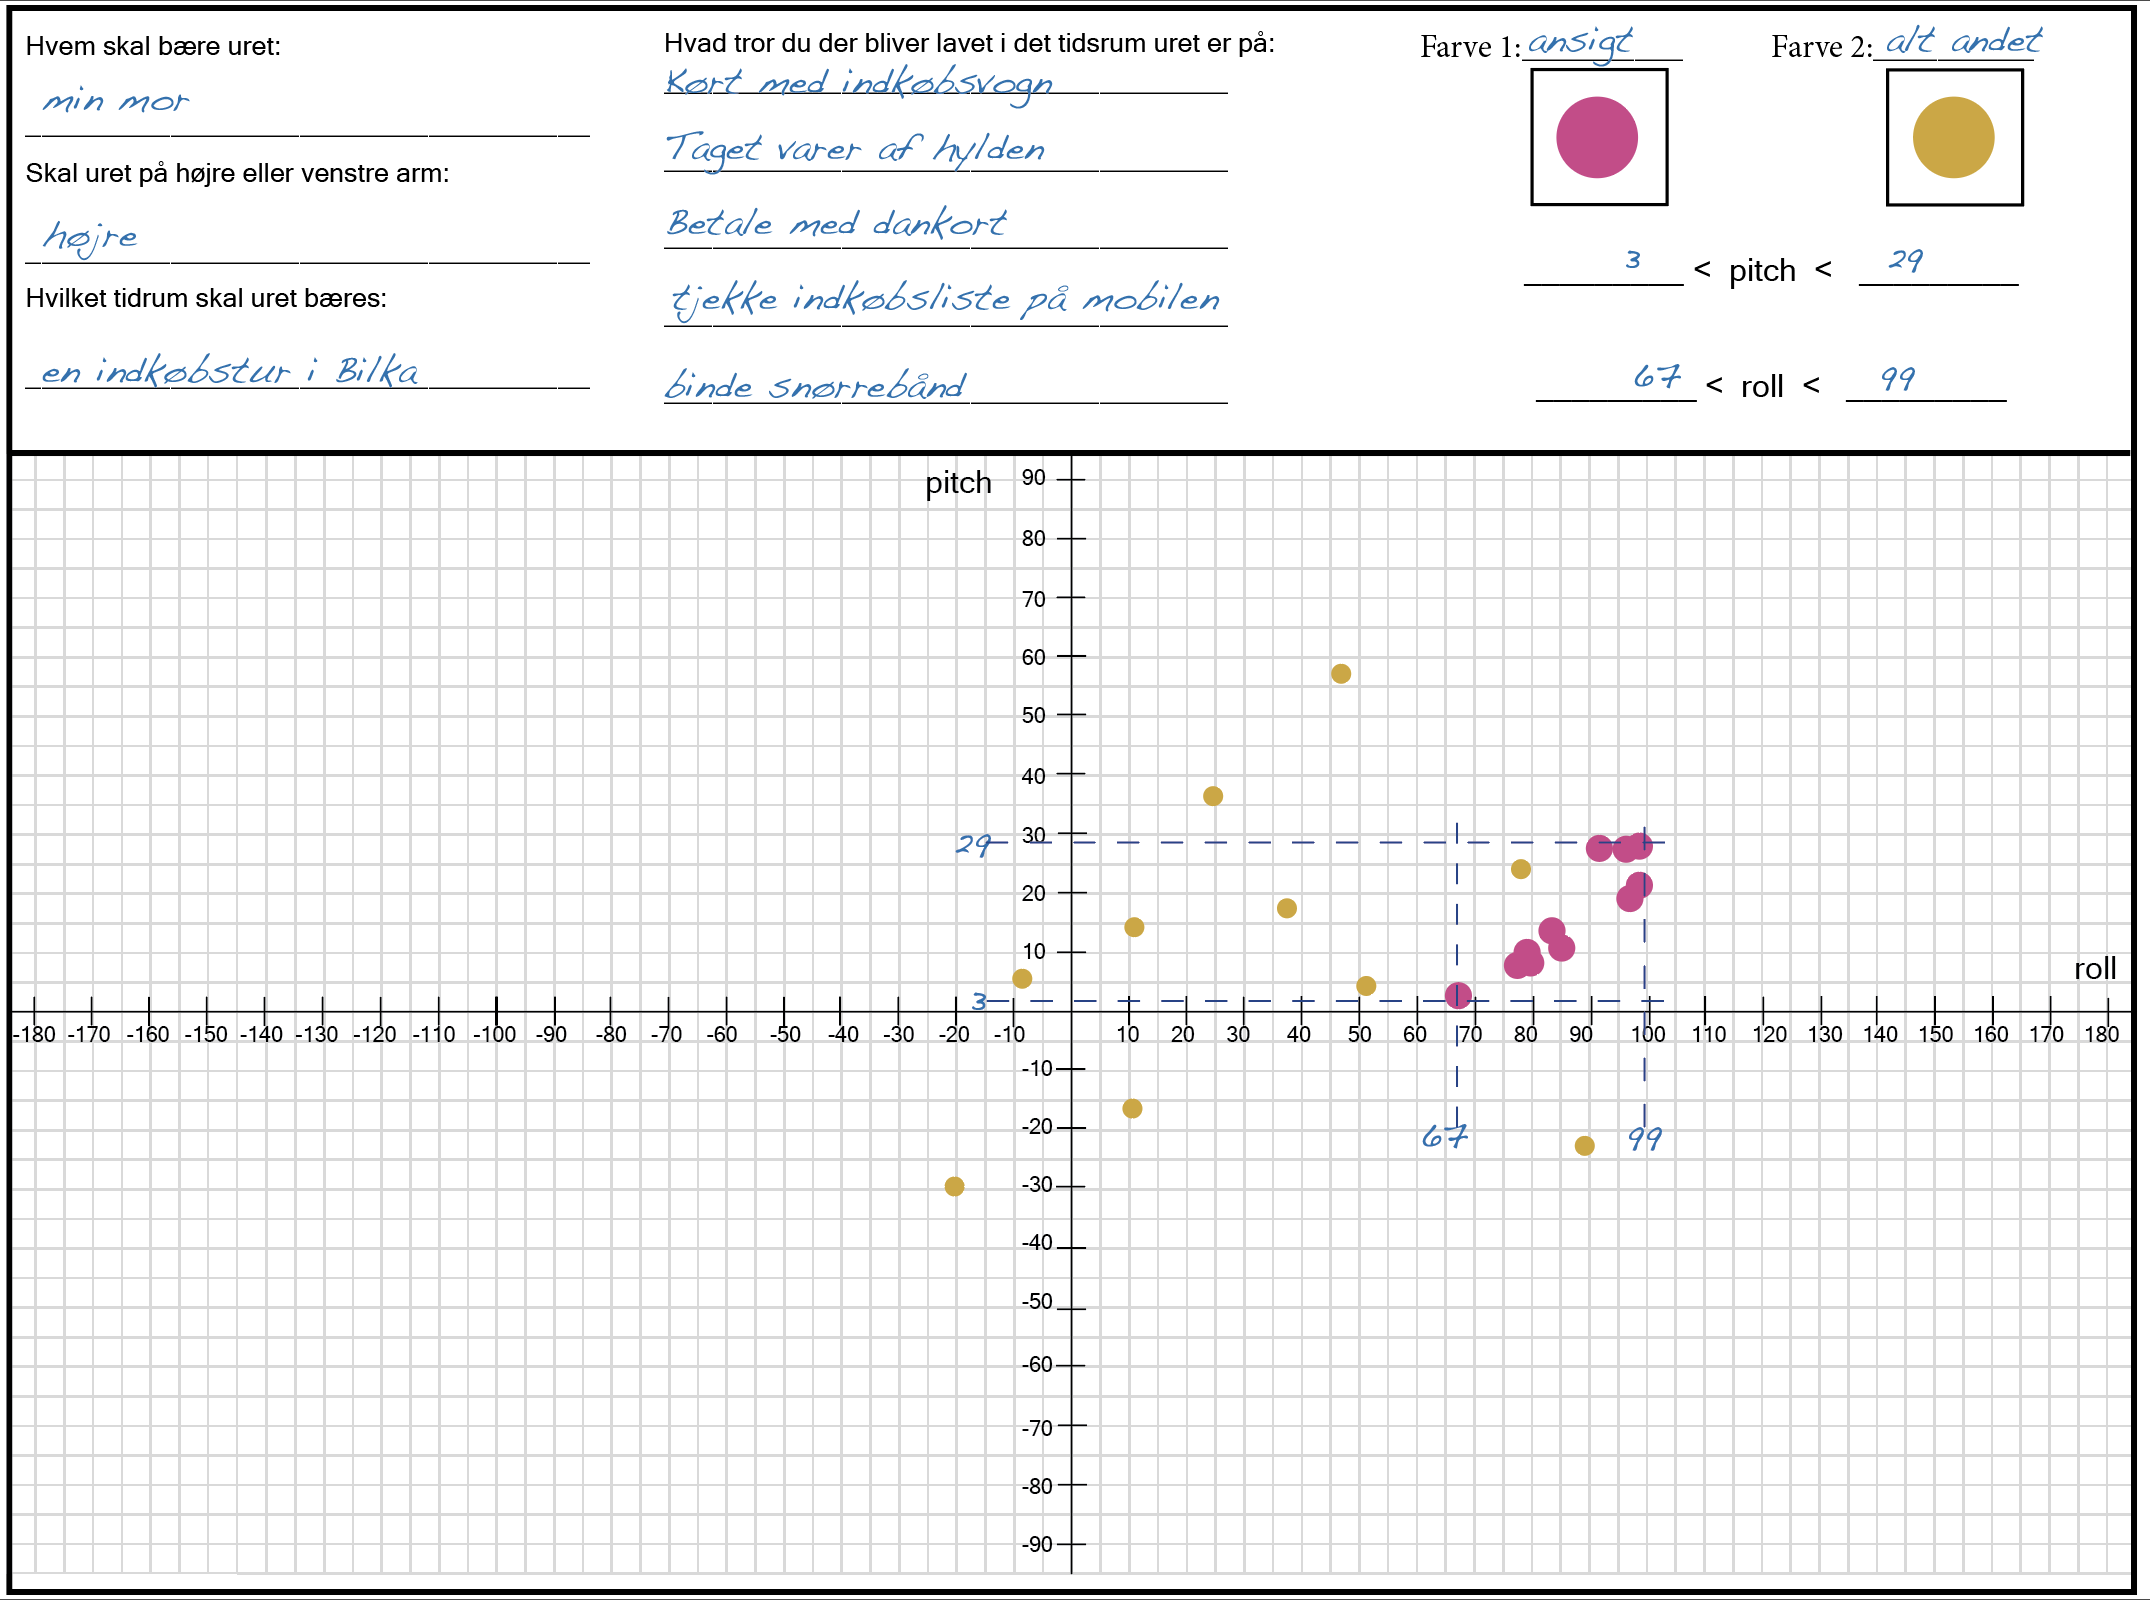
\includegraphics[width=1\textwidth]{billeder/coronaansigt.png}

Tag det udleverede ark med koordinatsystemet og to tusher i hver sin farve. \\

Snak om hvem der skal have uret på når det skal med hjem - og prøve at regne ud om uret skal sidde på venstre eller højre hånd for at få det mest brugbare resultat. \\

En af jer skal nu have uret på og lade som om hen kigger på sin mobil. Den anden notere i koordinatsystemet på arket ved at sætte en prik. Prøv lidt forskellige håndstillinger og noter mindst 10 punkter.\\

Tag den anden farve og gør det samme, men forstil jer at I laver alt muligt andet end at kigge på en mobil. F.eks, skriver på computer, drikker af en kop, tømmer vaskemaskinen, eller andre aktiviteter I forstiller jer at jeres testperson kunne udføre. Hvis nogen af de prikker I sætter her, kommer tæt på de prikker I satte for mobilbrug, så lav gerne en lille note, så I kan huske hvad den aktivitet var. \\

Byt om, så den der ikke havde uret på før, har uret på og den anden skriver ned. \\ 

Når I begge har et udfyldt koordinatsystem, skal I ramme tallene for mobil-kiggeriet ind og forlænge linjerne til de møder x og y-aksen. I kan nu aflæse det interval jeres mobil-forbrug-data ligger indefor. Noter det på arket ved hjælp af uligheder.  

\end{exercisebox}

\end{document}
